\documentclass[aspectratio=169,11pt]{beamer}

% -----------------------------------------------------------------------------
% Theme and colours
% -----------------------------------------------------------------------------
\usetheme[progressbar=frametitle, numbering=fraction, block=fill, background=light]{metropolis}

% A refined accent palette
\definecolor{IronDark}{HTML}{1A2B3C}
\definecolor{IronBlue}{HTML}{2E86AB}
\definecolor{IronTeal}{HTML}{06A77D}
\definecolor{IronOrange}{HTML}{F18F01}
\definecolor{IronRed}{HTML}{C73E1D}
\definecolor{IronLight}{HTML}{F4F7F9}
\definecolor{IronGray}{HTML}{5D6D7E}

\setbeamercolor{frametitle}{bg=IronDark, fg=white}
\setbeamercolor{progress bar}{fg=IronTeal}
\setbeamercolor{title}{fg=IronDark}
\setbeamercolor{subtitle}{fg=IronGray}
\setbeamercolor{author}{fg=IronGray}
\setbeamercolor{institute}{fg=IronGray}
\setbeamercolor{date}{fg=IronGray}
\setbeamercolor{block title}{bg=IronBlue, fg=white}
\setbeamercolor{block body}{bg=IronBlue!8, fg=IronDark}
\setbeamercolor{block title alerted}{bg=IronRed, fg=white}
\setbeamercolor{block body alerted}{bg=IronRed!8, fg=IronDark}
\setbeamercolor{block title example}{bg=IronTeal, fg=white}
\setbeamercolor{block body example}{bg=IronTeal!8, fg=IronDark}
\setbeamercolor{item}{fg=IronBlue}
\setbeamercolor{subitem}{fg=IronTeal}
\setbeamercolor{caption name}{fg=IronBlue}

\metroset{sectionpage=progressbar, subsectionpage=none}

% -----------------------------------------------------------------------------
% Packages
% -----------------------------------------------------------------------------
\usepackage{tikz}
\usetikzlibrary{arrows.meta,positioning,shapes.multipart,fit,shadows.blur}
\usepackage{booktabs}
\usepackage{array}
\usepackage{fontawesome5}
\usepackage{etoolbox}

% Remove navigation symbols
\setbeamertemplate{navigation symbols}{}

% -----------------------------------------------------------------------------
% Metadata
% -----------------------------------------------------------------------------
\title{IronClaw}
\subtitle{Dynamic Tool Synthesis and Secure MicroVM Isolation for Autonomous Agents}
\author{Suryavir Kapur}
\institute{BITS Pilani \quad\(\cdot\)\quad Supervisor: Dr.~Vijaykumar B.}
\date{July 2026}

% -----------------------------------------------------------------------------
% TikZ styles consistent with the colour palette
% -----------------------------------------------------------------------------
\tikzset{
  box/.style={draw=IronDark, rounded corners=4pt, align=center, minimum height=0.9cm, minimum width=2.3cm, fill=IronLight, line width=0.8pt, font=\small},
  host/.style={draw=IronTeal, rounded corners=4pt, align=center, minimum height=0.9cm, minimum width=2.5cm, fill=IronTeal!10, line width=0.8pt, font=\small},
  guest/.style={draw=IronOrange, rounded corners=4pt, align=center, minimum height=0.9cm, minimum width=2.5cm, fill=IronOrange!12, line width=0.8pt, font=\small},
  warn/.style={draw=IronRed, rounded corners=4pt, align=center, minimum height=0.9cm, minimum width=2.5cm, fill=IronRed!10, line width=0.8pt, font=\small},
  arrow/.style={-{Latex[length=2.5mm,width=1.8mm]}, thick, IronDark},
  label/.style={font=\footnotesize\color{IronGray}}
}

% -----------------------------------------------------------------------------
% Document
% -----------------------------------------------------------------------------
\begin{document}

% Title frame
\begin{frame}[plain]
  \begin{tikzpicture}[remember picture,overlay]
    % Split background and architectural accents
    \fill[IronLight] (current page.south west) rectangle (current page.north east);
    \fill[IronDark]
      ([xshift=-0.32\paperwidth]current page.south east)
      rectangle (current page.north east);
    \fill[IronTeal]
      ([xshift=-0.32\paperwidth]current page.south east)
      rectangle ([xshift=-0.315\paperwidth]current page.north east);
    \fill[IronOrange]
      ([xshift=-0.32\paperwidth,yshift=0.55cm]current page.south east)
      rectangle ([xshift=-0.23\paperwidth,yshift=0.63cm]current page.south east);

    % Thesis label
    \node[
      anchor=north west,
      fill=IronTeal,
      text=white,
      rounded corners=2pt,
      inner xsep=8pt,
      inner ysep=4pt,
      font=\scriptsize\bfseries
    ] at ([xshift=0.85cm,yshift=-0.65cm]current page.north west)
      {UNDERGRADUATE THESIS \(\cdot\) BITS F423T};

    % Main title block
    \node[
      anchor=north west,
      align=left,
      text width=0.58\paperwidth,
      text=IronDark
    ] at ([xshift=0.85cm,yshift=-1.45cm]current page.north west) {
      {\fontsize{27}{30}\selectfont\bfseries IronClaw}\\[0.18cm]
      {\fontsize{15}{18}\selectfont
        Dynamic Tool Synthesis\\
        and Secure \mbox{MicroVM} Isolation}\\[-0.02cm]
      {\fontsize{12}{15}\selectfont\color{IronGray}
        for Autonomous Agents}
    };

    % Contribution pills
    \node[
      anchor=west,
      draw=IronBlue,
      fill=IronBlue!8,
      text=IronDark,
      rounded corners=4pt,
      inner xsep=8pt,
      inner ysep=5pt,
      font=\small
    ] at ([xshift=0.85cm,yshift=2.50cm]current page.south west)
      {\faCogs\quad Synthesize once, reuse safely};
    \node[
      anchor=west,
      draw=IronOrange,
      fill=IronOrange!9,
      text=IronDark,
      rounded corners=4pt,
      inner xsep=8pt,
      inner ysep=5pt,
      font=\small
    ] at ([xshift=0.85cm,yshift=1.73cm]current page.south west)
      {\faLock\quad Contain generated code in Firecracker};

    % Author information
    \node[
      anchor=south west,
      align=left,
      text=IronGray,
      font=\scriptsize
    ] at ([xshift=0.85cm,yshift=0.42cm]current page.south west) {
      \textbf{\color{IronDark}Suryavir Kapur}
      \(\;\cdot\;\) 2022A7TS0293U
      \(\;\cdot\;\) July 2026\\
      Supervisor: Dr.~Vijaykumar B.
    };

    % BITS identity panel
    \node[
      fill=white,
      rounded corners=8pt,
      inner sep=8pt
    ] at ([xshift=0.34\paperwidth,yshift=0.65cm]current page.center)
      {
\includegraphics[width=2.75cm]{Pictures/bits_logo.png}};
    \node[
      anchor=north,
      align=center,
      text=white,
      text width=0.27\paperwidth,
      font=\scriptsize
    ] at ([xshift=0.34\paperwidth,yshift=-1.2cm]current page.center) {
      \textbf{\normalsize BITS Pilani}\\[0.08cm]
      Department of Computer Science\\
      \& Information Systems
    };
  \end{tikzpicture}
\end{frame}

% =============================================================================
\section{Architecture Summary}
% =============================================================================

\begin{frame}{IronClaw Architecture}
  \centering
  \resizebox{0.98\textwidth}{!}{%
  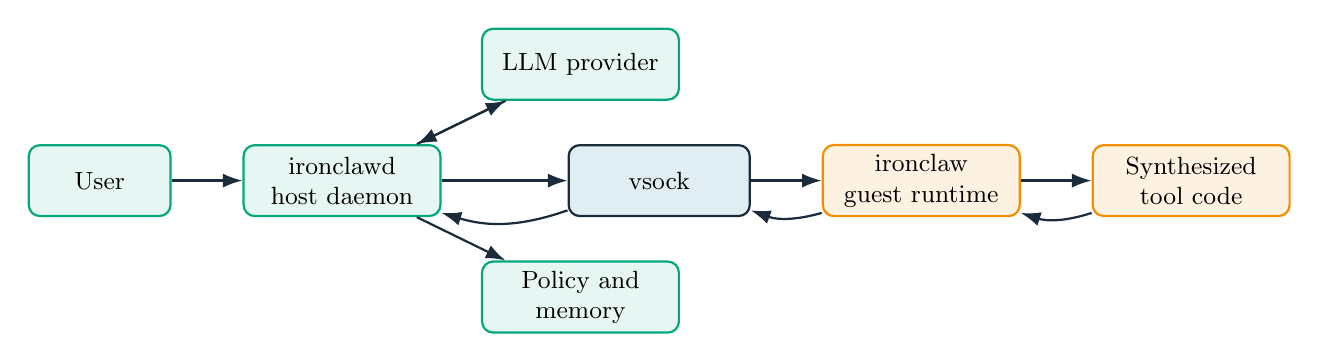
\begin{tikzpicture}[node distance=0.7cm]
    \node[host, minimum width=1.8cm] (user) {User};
    \node[host, right=0.9cm of user] (daemon) {ironclawd\\host daemon};
    \node[host, above right=0.55cm and 0.5cm of daemon] (llm) {LLM provider};
    \node[host, below right=0.55cm and 0.5cm of daemon] (policy) {Policy and\\memory};
    \node[box, right=1.6cm of daemon, fill=IronBlue!15] (vsock) {vsock};
    \node[guest, right=0.9cm of vsock] (guest) {ironclaw\\guest runtime};
    \node[guest, right=0.9cm of guest] (tool) {Synthesized\\tool code};

    \draw[arrow] (user) -- (daemon);
    \draw[arrow] (daemon) -- (llm);
    \draw[arrow] (llm) -- (daemon);
    \draw[arrow] (daemon) -- (policy);
    \draw[arrow] (daemon) -- (vsock);
    \draw[arrow] (vsock) -- (guest);
    \draw[arrow] (guest) -- (tool);
    \draw[arrow] (tool) to[bend left=18] (guest);
    \draw[arrow] (guest) to[bend left=18] (vsock);
    \draw[arrow] (vsock) to[bend left=18] (daemon);
  \end{tikzpicture}%
  }
  \vspace{0.15cm}

  \small Trusted Rust host plans and gates; generated code runs inside a
  disposable Firecracker microVM reached only over vsock.
\end{frame}

\begin{frame}{Architecture Summary: Trusted Host, Disposable Guest}
  \scriptsize
  \begin{columns}[T,totalwidth=\textwidth]
    \begin{column}{0.48\textwidth}
      \begin{block}{\faServer\ Host daemon (trusted)}
        \begin{itemize}
          \item Task intake API and plan--act--observe agent loop with the
            prompt/provider layer.
          \item Policy manager gates every dispatch; sandbox supervisor owns
            the VM lifecycle.
          \item Memory, logs, and result triage stay on the host.
        \end{itemize}
      \end{block}
    \end{column}
    \begin{column}{0.48\textwidth}
      \begin{exampleblock}{\faLock\ Guest runtime (untrusted)}
        \begin{itemize}
          \item Validate envelope \(\rightarrow\) materialize inputs
            \(\rightarrow\) run tool with limits.
          \item Capture stdout, stderr, and exit status; return a structured
            response.
          \item Sees only the inputs explicitly sent for the current execution.
        \end{itemize}
      \end{exampleblock}
    \end{column}
  \end{columns}
  \vspace{0.25cm}
  \centering
  \textbf{Split of trust:} the host owns planning, policy, providers, lifecycle
  control, and triage; the guest only executes.
\end{frame}

\begin{frame}{Architecture Summary: Envelope, Lifecycle, Policy}
  \centering
  \resizebox{0.9\textwidth}{!}{%
  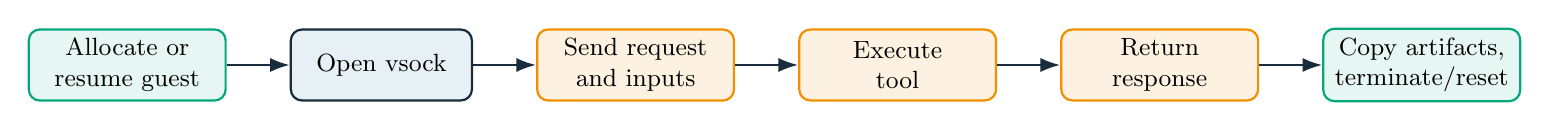
\begin{tikzpicture}[node distance=0.8cm, every node/.style={font=\scriptsize}]
    \node[host] (alloc) {Allocate or\\resume guest};
    \node[box, right=of alloc, fill=IronBlue!12] (vsock) {Open vsock};
    \node[guest, right=of vsock] (send) {Send request\\and inputs};
    \node[guest, right=of send] (exec) {Execute\\tool};
    \node[guest, right=of exec] (resp) {Return\\response};
    \node[host, right=of resp] (reset) {Copy artifacts,\\terminate/reset};

    \draw[arrow] (alloc) -- (vsock);
    \draw[arrow] (vsock) -- (send);
    \draw[arrow] (send) -- (exec);
    \draw[arrow] (exec) -- (resp);
    \draw[arrow] (resp) -- (reset);
  \end{tikzpicture}%
  }
  \vspace{0.25cm}

  \scriptsize
  \begin{columns}[T,totalwidth=\textwidth]
    \begin{column}{0.32\textwidth}
      \begin{block}{Request envelope}
        request id, tool name, generated code/command, serialized inputs,
        resource limits, expected result format.
      \end{block}
    \end{column}
    \begin{column}{0.32\textwidth}
      \begin{block}{Response envelope}
        status, exit code, duration, bounded stdout/stderr, artifact metadata,
        error classification.
      \end{block}
    \end{column}
    \begin{column}{0.32\textwidth}
      \begin{alertblock}{Policy and failures}
        interpreter allowlist, file/network mode, CPU/memory/time limits,
        output truncation; errors classified (tool, policy, timeout,
        transport).
      \end{alertblock}
    \end{column}
  \end{columns}
\end{frame}

% =============================================================================
\section{Hypotheses}
% =============================================================================

\begin{frame}{Hypotheses}
  \begin{block}{H1: Utility}
    On repeated tasks for which no purpose-built tool is available,
    policy-guided dynamic tool synthesis reduces model interaction steps and
    token consumption relative to generic capabilities alone, while preserving
    task correctness. \textbf{The benefit increases with reuse.}
  \end{block}
  \vspace{0.35cm}
  \begin{exampleblock}{H2: Security and Performance}
    IronClaw's microVM architecture contains simulated host-breakout attempts
    from malicious synthesized tools, at the cost of measurable but acceptable
    initialization latency and memory overhead.
  \end{exampleblock}
\end{frame}

% =============================================================================
\section{Results}
% =============================================================================

\begin{frame}{H1 Setup: One Mechanism, Three Domains, Five Experiments}
  \scriptsize
  \begin{columns}[T,totalwidth=\textwidth]
    \begin{column}{0.47\textwidth}
      \begin{block}{A: No synthesis}
        Agent authors the required SQL/JavaScript inline; the logic is
        produced again for every request.
      \end{block}
      \vspace{0.12cm}
      \begin{exampleblock}{B: Dynamic synthesis}
        Same base capability plus one meta-tool that registers generated
        logic: create once, then reuse with small inputs.
      \end{exampleblock}
      \vspace{0.12cm}
      \begin{block}{Held constant / acceptance}
        \texttt{deepseek-v4-pro}, settings, seeded fixtures, request order,
        validation, metric code. B must preserve correctness and cut
        steps/tokens on repeated work.
      \end{block}
    \end{column}
    \begin{column}{0.50\textwidth}
      \renewcommand{\arraystretch}{1.28}
      \begin{tabular}{clc}
        \toprule
        \textbf{ID} & \textbf{Domain (repeated artifact)} & \textbf{Reuse} \\
        \midrule
        E1 & SQL: seven-table cancellation query & 6/6 \\
        E2 & SQL: sparse-reuse variant & 3/6 \\
        E3 & Parser: hostile legacy log files & 6/6 \\
        E4 & Parser: sparse-reuse variant & 3/6 \\
        E5 & Repository: seven-rule compliance audit & 6/6 \\
        \bottomrule
      \end{tabular}
      \vspace{0.25cm}

      Each A/B condition is one six-request conversation --- ten measured
      conversations in total. The design tests both benefit and break-even
      behavior.
    \end{column}
  \end{columns}
\end{frame}

\begin{frame}{H1 Results: Repetitive Workloads}
  \centering
  \footnotesize
  \renewcommand{\arraystretch}{1.22}
  \begin{tabular}{lrrrc}
    \toprule
    \textbf{Domain} & \textbf{A input} & \textbf{B input} & \textbf{Change} & \textbf{Correct} \\
    \midrule
    E1: SQL & 190{,}031 & \textbf{88{,}566} & $-$53.4\% & 100\% / 100\% \\
    E3: parser & 193{,}817 & \textbf{74{,}865} & $-$61.4\% & 100\% / 100\% \\
    E5: repository audit & 140{,}472 & \textbf{65{,}146} & $-$53.6\% & 100\% / 100\% \\
    \bottomrule
  \end{tabular}
  \vspace{0.35cm}
  \begin{exampleblock}{Primary result}
    With six repeated uses, synthesis reduced billed input tokens by
    \textbf{53--61\%} without changing answer correctness.
  \end{exampleblock}
  \vspace{0.15cm}
  \footnotesize
  Input-token totals include the entire growing conversation and every
  intermediate tool-loop step---the units that are actually billed.
\end{frame}

\begin{frame}{H1 Results: Why the Token Reduction Occurred}
  \scriptsize
  \renewcommand{\arraystretch}{1.18}
  \setlength{\tabcolsep}{3pt}
  \begin{tabular}{lrrrrrr}
    \toprule
    & \multicolumn{2}{c}{\textbf{Model steps}} &
      \multicolumn{2}{c}{\textbf{Code chars}} &
      \multicolumn{2}{c}{\textbf{Wall time}} \\
    \textbf{Domain} & A & B & A & B & A & B \\
    \midrule
    SQL & 28 & 15 & 3{,}142 & 1{,}800 & 103.6\,s & 81.3\,s \\
    Parser & 18 & 13 & 6{,}109 & 1{,}196 & 91.7\,s & 47.2\,s \\
    Repository & 19 & 13 & 29{,}176 & 9{,}112 & 134.0\,s & 61.4\,s \\
    \bottomrule
  \end{tabular}
  \vspace{0.28cm}
  \begin{columns}[T,totalwidth=\textwidth]
    \begin{column}{0.48\textwidth}
      \begin{block}{A repeatedly pays}
        Rediscover/restate logic $\rightarrow$ author code $\rightarrow$ execute
        it, with the growing transcript resent at later model steps.
      \end{block}
    \end{column}
    \begin{column}{0.48\textwidth}
      \begin{exampleblock}{B pays once, then reuses}
        Create and register the artifact, then later requests send small
        parameters to deterministic code.
      \end{exampleblock}
    \end{column}
  \end{columns}
\end{frame}

\begin{frame}{H1 Results: Sparse Reuse Is Net-Negative}
  \footnotesize
  \begin{columns}[T,totalwidth=\textwidth]
    \begin{column}{0.43\textwidth}
      \centering
      \renewcommand{\arraystretch}{1.25}
      \begin{tabular}{lrr}
        \toprule
        \textbf{Input tokens} & \textbf{A} & \textbf{B} \\
        \midrule
        E2: SQL & 73{,}452 & 87{,}442 \\
        E4: parser & 64{,}452 & 106{,}131 \\
        \bottomrule
      \end{tabular}
      \vspace{0.3cm}

      E2: \alert{+19.0\%}\\
      E4: \alert{+64.7\%}
    \end{column}
    \begin{column}{0.53\textwidth}
      \begin{alertblock}{Why B loses at 3/6}
        \begin{enumerate}
          \item Creating a tool requires extra code and model steps.
          \item That creation transcript remains in later context.
          \item Only two later requests reuse the created artifact.
          \item The saved inline work does not repay the creation/context cost.
        \end{enumerate}
      \end{alertblock}
    \end{column}
  \end{columns}
  \vspace{0.2cm}
  \begin{block}{What can and cannot be concluded}
    In these workloads, 3/6 loses and 6/6 wins. The exact break-even lies
    somewhere between them, but is task/model dependent and was not estimated.
  \end{block}
\end{frame}

\begin{frame}{H1 Design Lesson: Keep Bulk Data Behind the Tool}
  \footnotesize
  \begin{columns}[T,totalwidth=\textwidth]
    \begin{column}{0.46\textwidth}
      \begin{alertblock}{Initial parser design}
        Created tool receives the \emph{entire log text} as an argument.
        \begin{itemize}
          \item Bulk input enters the model/tool transcript.
          \item Dynamic condition: \alert{+12\% input tokens}.
        \end{itemize}
      \end{alertblock}
    \end{column}
    \begin{column}{0.46\textwidth}
      \begin{exampleblock}{Final controlled design}
        Created tool receives a small filename and uses allow-listed
        \texttt{readFile(name)}.
        \begin{itemize}
          \item Data stays behind the capability boundary.
          \item Dynamic condition: \textbf{$-$61.4\%}.
        \end{itemize}
      \end{exampleblock}
    \end{column}
  \end{columns}
  \vspace{0.3cm}
  \centering
  \Large\textbf{Pass lookup keys, not bulk data.}
\end{frame}

\begin{frame}{H1 Answer}
  \begin{exampleblock}{Supported within the tested conditions}
    Dynamic synthesis preserved 100\% correctness and reduced input tokens,
    model steps, authored code, and wall time when the same complex operation
    was reused across all six requests.
  \end{exampleblock}
  \vspace{0.25cm}
  \begin{alertblock}{Not universally beneficial}
    When only three of six requests required the capability, synthesis increased
    input tokens by 19.0--64.7\%; creation was not amortized.
  \end{alertblock}
  \vspace{0.3cm}
  \centering
  \textbf{Decision rule for IronClaw:}\\
  synthesize when repeated reuse is expected; otherwise execute inline.
\end{frame}

\begin{frame}{H2 Setup: Boundary Comparison and Five Host Targets}
  \scriptsize
  \begin{columns}[T,totalwidth=\textwidth]
    \begin{column}{0.44\textwidth}
      \begin{alertblock}{Process baseline}
        Child shell runs directly on the host with the invoking user's
        permissions.
      \end{alertblock}
      \vspace{0.12cm}
      \begin{exampleblock}{Firecracker condition}
        Identical command runs inside a guest through IronClaw's production
        manager, authentication, protobuf, and vsock path.
      \end{exampleblock}
      \vspace{0.12cm}
      \begin{block}{Environment and scope}
        i7-12700K; Firecracker 1.14.0; guest Linux 6.1.155 + Ubuntu 24.04;
        2 vCPU, 512\,MiB. Networking disabled; tests filesystem, environment,
        device, and namespace containment.
      \end{block}
    \end{column}
    \begin{column}{0.52\textwidth}
      \renewcommand{\arraystretch}{1.22}
      \begin{tabular}{>{\raggedright\arraybackslash}p{0.32\columnwidth}
                      >{\raggedright\arraybackslash}p{0.60\columnwidth}}
        \toprule
        \textbf{Payload} & \textbf{What the command attempts} \\
        \midrule
        Host file read & Read a random sentinel file created only on the host \\
        Host file write & Create a marker inside a host-only directory \\
        Environment read & Read a random host-only environment variable \\
        Device access & Detect the host's \texttt{/dev/kvm} \\
        Namespace observe & Read the host hostname through \texttt{/proc} \\
        \bottomrule
      \end{tabular}
      \vspace{0.2cm}

      Breakout \(=\) the targeted \emph{host} resource is observed or
      modified.\\[0.1cm]
      \textbf{Security criterion:} 0/5 host-resource accesses in
      Firecracker.\\[0.1cm]
      \textbf{Init target:} $t_{\text{init}}<500$\,ms for snapshot-resumed
      guests; cold boot is reported separately and does not test this target.
    \end{column}
  \end{columns}
\end{frame}

\begin{frame}{H2 Security Result: 5/5 vs 0/5}
  \centering
  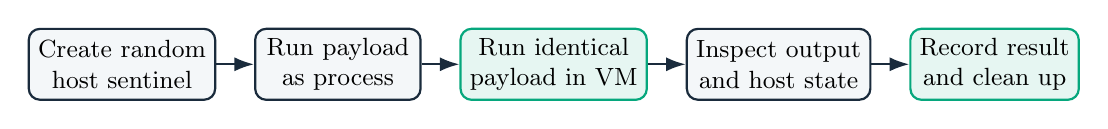
\begin{tikzpicture}[node distance=0.48cm, every node/.style={font=\scriptsize}]
    \node[box, minimum width=2.1cm] (sentinel) {Create random\\host sentinel};
    \node[box, right=of sentinel, minimum width=2.1cm] (process) {Run payload\\as process};
    \node[host, right=of process, minimum width=2.1cm] (vm) {Run identical\\payload in VM};
    \node[box, right=of vm, minimum width=2.1cm] (verify) {Inspect output\\and host state};
    \node[host, right=of verify, minimum width=2.1cm] (cleanup) {Record result\\and clean up};
    \draw[arrow] (sentinel) -- (process);
    \draw[arrow] (process) -- (vm);
    \draw[arrow] (vm) -- (verify);
    \draw[arrow] (verify) -- (cleanup);
  \end{tikzpicture}
  \vspace{0.35cm}
  \small
  \renewcommand{\arraystretch}{1.13}
  \begin{tabular}{lccc}
    \toprule
    \textbf{Target} & \textbf{Process attack} & \textbf{VM attack} & \textbf{Contained} \\
    \midrule
    file read / file write & 2/2 succeeded & 0/2 succeeded & 2/2 \\
    environment / device & 2/2 succeeded & 0/2 succeeded & 2/2 \\
    namespace observation & 1/1 succeeded & 0/1 succeeded & 1/1 \\
    \midrule
    \textbf{Total} & \alert{\textbf{5/5}} & \textbf{0/5} & \textbf{5/5} \\
    \bottomrule
  \end{tabular}
\end{frame}

\begin{frame}{H2 Performance Results}
  \scriptsize
  \renewcommand{\arraystretch}{1.16}
  \setlength{\tabcolsep}{4pt}
  \begin{tabular}{lrr}
    \toprule
    \textbf{Metric} & \textbf{Process} & \textbf{Firecracker} \\
    \midrule
    Start/cold median (p95) & 36.45\,ms (94.00) & 6{,}083.67\,ms (6{,}102.59) \\
    Warm no-op median (p95) & 36.45\,ms (94.00) & 1.74\,ms (3.68) \\
    Host resident memory & 4{,}108\,KiB & 72{,}672\,KiB \\
    Configured guest memory & --- & 512\,MiB \\
    CPU-loop utilization & 92.2\% & 99.6\% \\
    Stop + restart + probe median (p95) & --- & 6{,}622.87\,ms (6{,}632.47) \\
    \bottomrule
  \end{tabular}
  \vspace{0.24cm}
  \begin{columns}[T,totalwidth=\textwidth]
    \begin{column}{0.48\textwidth}
      \begin{alertblock}{Dominant cost}
        Cold boot is approximately \textbf{167$\times$} process start and uses
        roughly 67\,MiB more host RSS; recovery succeeded 5/5 at 6.62\,s.
      \end{alertblock}
    \end{column}
    \begin{column}{0.48\textwidth}
      \begin{exampleblock}{Steady state}
        Cold start is a per-session lifecycle cost, amortized over many tool
        calls; warm 1.74\,ms reuses an existing guest, so it is not directly
        comparable to process creation.
      \end{exampleblock}
    \end{column}
  \end{columns}
  \vspace{0.12cm}
  \centering
  Fits long-lived tenant sessions, not interactive per-request VM creation.
\end{frame}

\begin{frame}{H2 Answer}
  \begin{exampleblock}{Containment component supported}
    All five attacks reached their host target under process execution; none
    reached it through the Firecracker boundary.
  \end{exampleblock}
  \vspace{0.25cm}
  \begin{alertblock}{Initialization overhead: bounded for long-lived VMs}
    Cold start (6.08\,s) and recovery (6.62\,s) are too slow for per-request
    isolation but acceptable for long-lived tenant sessions. The
    $<500$\,ms target applies to snapshot resume, which is not implemented,
    so it remains \emph{unevaluated}, not failed.
  \end{alertblock}
  \vspace{0.3cm}
  \centering
  \Large\textbf{H2 is partially supported.}
\end{frame}

\begin{frame}{Validity Limits and Future Extensions}
  \scriptsize
  \begin{columns}[T,totalwidth=\textwidth]
    \begin{column}{0.50\textwidth}
      \begin{alertblock}{What the evidence does not prove}
        \begin{itemize}
          \item H1: one model, one measured run per condition, two reuse
            frequencies; exact break-even not identified.
          \item H2: one host/VM configuration; five non-destructive payloads
            are not a proof of no vulnerabilities; network, fuzzing, side
            channels excluded; baseline is an unisolated process.
        \end{itemize}
      \end{alertblock}
      \vspace{0.15cm}
      \begin{exampleblock}{Bounded claim}
        The experiments establish the measured effect for these conditions;
        no universal token savings or complete microVM security is claimed.
      \end{exampleblock}
    \end{column}
    \begin{column}{0.46\textwidth}
      \begin{block}{\faHourglassHalf\ Future extensions}
        \begin{itemize}
          \item Snapshot create/restore and $<500$\,ms resume measurement.
          \item TAP-layer network allow-lists.
          \item Broader fuzzing; seccomp/container/WASM baselines.
          \item Larger benchmarks, more models, repeated trials.
        \end{itemize}
      \end{block}
    \end{column}
  \end{columns}
\end{frame}

\begin{frame}{Publishing Avenue}
  \begin{exampleblock}{\faBullseye\ Target venue}
    \textbf{ACM Transactions on AI Security and Privacy (TAISAP)}
  \end{exampleblock}
  \vspace{0.3cm}
  \footnotesize
  \begin{itemize}
    \item The evaluation pairs an AI-utility claim (H1, dynamic tool
      synthesis) with a security/systems claim (H2, microVM containment and
      overhead).
    \item TAISAP's scope covers AI systems evaluated under security and
      privacy constraints, matching the IronClaw contribution profile.
    \item Planned submission after extending the security suite and adding
      snapshot-resume measurements.
  \end{itemize}
\end{frame}

\begin{frame}{Thank You}
  \centering
  \Huge\textbf{Questions?}\\[0.6cm]
  \large\color{IronGray} Suryavir Kapur \(\cdot\) BITS Pilani\\
  \texttt{2022A7TS0293U}
\end{frame}

\end{document}
